\documentclass{article}[11pt]
\textheight 8.5in
\usepackage{graphicx}
\usepackage{float}%for forcing position of figs
\usepackage{hyperref}
\usepackage{amsmath}

\begin{document}
\begin{center}
Siddharthan Rajasekaran\\
Week of 3/06/2017 - 3/13/2017
\end{center}

\section{Summary of Discussions}
In this report, we will talk about the initial implementation of Apprenticeship Learning via Inverse Reinforcement Learning. In the last section, I have added some plans for the next week with possible directions and questions. Please let me know if the plan requires any change. 

\section{Grid world}
We pick the same grid world given in \cite{abbeel2004apprenticeship} to implement a proof of concept. The grid has a dimension of $128 \times 128$ (2-D). This grid is further divided into macro cells of $16 \times 16$ grid cells. Hence there are $8\times8$ = 64 macro cells. Each cell is initialized with a random reward from $[-1,1]$. These reward values are stored in the weight vector $w$. The dimension of this weight vector is $(64\times 1)$. We have a indicator feature vector $\phi(x,y)$ which is again $(64\times 1)$ and $i^{th}$ dimension of it is $1$ if $(x,y)$ belongs to $i^{th}$ macro cell and $0$ otherwise. Using the weight and the feature vectors, the reward function can be written as $$R(x,y) = w^T\phi(x,y)$$. According to the constraints in the algorithm that the total reward can never exceed $1$, we normalize $w$ using $w := \frac{w}{||w||_1}$. Given this reward function (for any $w$) we can compute the optimal action under the reward using value iteration \cite{russell1995modern}.


\section{Projection Algorithm}
We use value iteration using the reward function that we generated and compute optimal policy $\pi^*$ from 10 different initial states. We use these optimal behaviors as demonstrations.
\begin{enumerate}
\item Pick a random policy $\pi^{(0)}$. Find the feature expectation $\mu(\pi^{(0)})$ under this policy. $\mu(\pi^{(0)}) = \textbf{E}[\sum_{t=0}^\infty\gamma^tR(s_t)|\pi^{(0)}]$. Take the best feature expectation $\bar{\mu} = \mu(\pi^{(0)})$. $i=1$
\item Pick {$w = \frac{\mu(\pi^*) - \bar{\mu}}{||\mu(\pi^*) - \bar{\mu}||_1}$} and find the optimal policy $\mu(\pi^{(1)})$ under the new $w$ using value iteration. 
\item Now we have two policies $\pi^{(0)}$ and $\pi^{(1)}$. We can mix these policies and hence obtain any policy \textbf{along the line joining the two} (convex combination). Pick the closest point (the foot of the perpendicular from of $\mu^*$ to the line joining  $\pi^{(0)}$ and $\pi^{(1)}$) as $\bar{\mu}$
\item $t = ||\mu^* - \bar{\mu}||_2$. If $t < \epsilon$ for some $\epsilon$, terminate. Else, go to step 2.

\end{enumerate}

Once we are done, we have a set of behaviors stored during the algorithm $\pi^{(i)}$ and their corresponding feature expectation $\mu^{(i)}$. We can find the closest point to expert's feature expectation $\mu^*$ by solving the following quadratic program.

\begin{align*}
\min_{\lambda,\mu} ||\mu^* &- \mu||_2 \\
s.t. \ \ \ \ \textbf{1}^T\lambda &= 1 \\
\sum_i \lambda_i\mu^{(i)} &= \mu
\end{align*}

Hence we have a behavior $\pi_{mixed} = \sum_i \lambda_i \pi^{(i)}$. Note that as the paper claims, it is this mixture of behaviors that makes us behave similar to the expert and not the actual retrieval of the reward function. In fact, we do not necessarily retrieve the reward function. One easy instance where this can be understood is acting from parts of state space where there is no demonstrations. Since we do not have any demonstrations in some parts, we do not know the experts feature expectation $\mu^*$ under their behavior. Hence there is no way to correct our behavior to stay close to that of the expert. 

\section{Thoughts on proof of convergence}
Given the closest feature expectation $\bar{\mu}$ to $\mu^*$, it is enough to prove that the new point $\mu^{(i)}$ will be in the half space 

This is because we want the foot of the perpendicular on line joining $\mu^{(i)}$ and $\bar{\mu}$ to be a convex combination of the two ($\mu^{(i)}$ and $\bar{\mu}$). This will make sure that we always make a progress towards $\mu^*$. Moreover, the beauty is, we are also making sure that the new feature $\mu^{(i)}$ is in in the required half space (Eq. \ref{halfspace} holds). We do this by maximizing the cumulative reward (by doing value iteration) which is nothing but (can be loosely written as) $$\max_{\mu^{(i)}}w^T\mu^{i}$$. The obvious choice is to pick a policy that gives raise to $\mu{(i)}$ such that its dot product with w is positive. An obvious proof of convergence has been reduced to the problem of given any vector $w$ one should be able to find a $\mu$ such that it has a positive inner product. The worst we can do however, if not positive, is to have a zero inner product ($\mu = 0$). 

\begin{align}
\label{halfspace}
(\mu^* - \bar{\mu})^T(&\mu^{(i)} -\bar{\mu}) > 0 \\
\label{inner}
(\mu^* - \bar{\mu})^T \mu^{(i)} &> (\mu^* - \bar{\mu})^T \bar{\mu}
\end{align} 
 Given $w = (\mu^* - \bar{\mu})$, the value iteration can be written as
 \begin{align*}
 \max_{\mu^{(i)}}(\mu^* - \bar{\mu})^T(\mu^{(i)} -\bar{\mu})\\
 \max_{\mu^{(i)}}(\mu^* - \bar{\mu})^T\mu^{(i)}
 \end{align*}
 
 Substituting this in \ref{inner}, we just need to make sure that we can find a $\mu^{(i)}$ which has a higher inner product with $w$ than $\bar{\mu}$. The worst case that can happen is that $\bar{\mu}$ is already at the maximum. In which case Eq.\ref{halfspace} will be strictly 0. And we no longer can improve our solution.  
 
Another interpretation is that, say we perform poorly in $j^{th}$ macro cell. And the feature expectation of expert is more than our policy at this cell. Now, this gives rise to a positive weight in $j^{th}$ dimension. Hence we might find a better policy near $j^{th}$ macro cell to have higher feature expectation. Implies that the expert wandered more in $j^{th}$ dimension so you better do that to. If we have a lesser feature expectation of the expert in $j^{th}$ dimension, then expert wandered less than us in that corresponding macro cell, so you better stay away from that too. Hence the difference in the feature expectations actually translates to a force that lets you be in a macro cell or not. Beautiful! 

\textbf{Another insight:} If we demonstrate sub-optimally, then during IRL we have to find a weight vector such that the optimal policy under the weight vector has the same sub-optimal feature expectations. This is impossible. Because given any feature vector the policy tries to exit every tile as soon as possible unless it is absorbing. To check this, we consider a policy that spans across 3 tiles (macro cells). We'll call them left, middle and right tiles. Our goal is to reach the right tile starting at the left one by crossing the middle tile. The optimal policy would just be taking the action 'East' at left and middle tiles. But we purposefully perform a sub optimal demonstration by taking two 'North' actions in the left tile. This increases our expectation of feature (in the dimension corresponding to the left tile). Hence starting from the left corner, we would optimally stay in left tile for 16 time steps (the length of the tile is 16 and after each action we cover one tile). But because of our sub optimal policy we stay in left tile for 18 time steps. The problem now is if the weight vector corresponding to left tile is increased, then we stay in left tile forever, or if it is decreased, we try to leave the left tile ASAP (in which case we spend only 16 time steps). Hence there is not one vector $w$ that encourages the system to stay in the tile for 18 time-steps (which is in between the extremes). 

Hence we get the following plot (Fig.\ref{fig:osc}) during our iterations to do IRL using SVM. Note that the weight component corresponding to the left tile is oscillating. In the algorithm, $w = \mu_E - \bar{\mu}$ ($\mu_E$ - feature expectation of expert, $\bar{\mu}$ - feature expectation with our best estimate of reward function). This oscillation means that setting $w$ to positive makes us spend more time than $18$ on left tile setting it to negative makes it spend $16$. The weight vector is hence oscillating in this dimension instead of converging. As a result the other dimension also oscillate in order to accomodate the change in left tile. The convergence however is due to the other feature dimensions that close in on $\mu_E$.

\begin{figure}[H]
  \begin{center}
    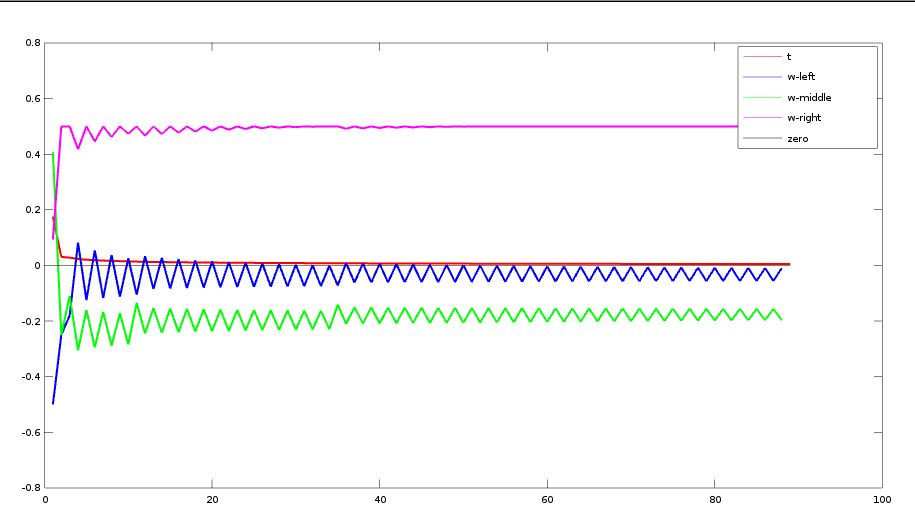
\includegraphics[width=1.2\linewidth]{images/osc}
    \caption{Oscillation in reward weights being learned}
    \label{fig:osc}
  \end{center}
\end{figure}

Finally we achieve a middle ground by mixing the policy. As the authors mention, in SVM IRL, our main aim is not to recover the weights but the policy. Mixing the feature expectations in the right proportions lets us get a mixed policy that has the expect features same as that of the expert. 

In case of sub optimal policy, we do not have one unique way of doing it. This is even true in case of optimal policy. For example, we talk about the 'L' shaped trajectory previously.

\subsection{Other Observations}
In case the demonstration is long, the actions at the end of the demonstrations do not affect the feature expectations as much. Hence, picking random actions towards the end of the demonstration is equally good for the agent just as in the beginning. For this one solution increasing the gamma. But this increases the time taken for value iteration. Is there a better way to do this other than increasing gamma? 

\subsection{Different ways to meet feature expectations}

Say the optimal agent behaves such that it takes and 'L' route towards a tile. Then there is many different ways to get to the tile than just taking the same 'L' which meets the same feature expectations. I think this is where MaxEnt comes in where we want to behave as randomly as possible while executing the 'L'.

Basically we hash the high dimensional behavior into the feature expectation using $\sum_t \gamma^t \phi_t$. Assuming that each behavior has unique has, and the hashing is bijective we can recover the true behavior. However, this is not the case, hence the backward mapping has to choose betwwen all the behaviors that can create the same hash. \textbf{Idea: Can we think of a bijective hash using irrational numbers (in gamma) that can be analytically inverted instead of iterative procedure?}
 
\section{Results of implementation}
\begin{figure}[H]
  \begin{center}
    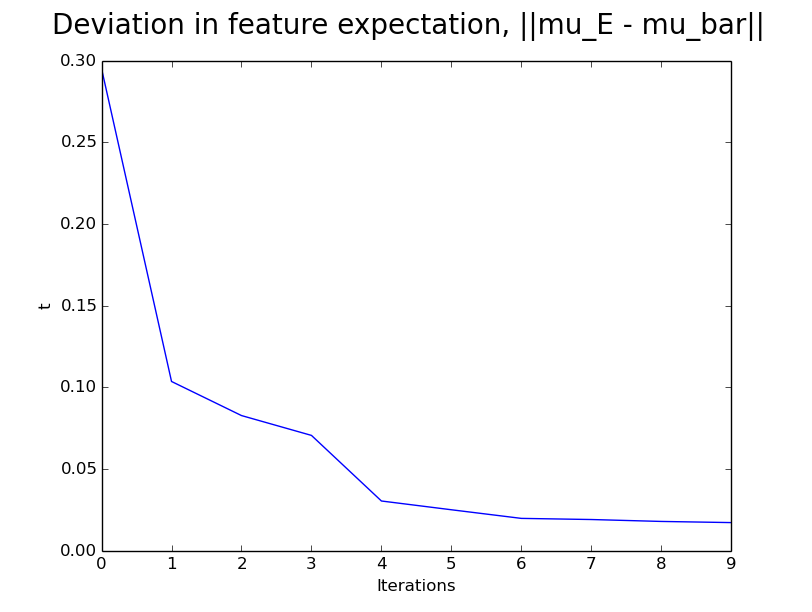
\includegraphics[width=0.9\linewidth]{images/figure_1}
    \caption{Deviation in feature expectation from the expert's behavior $\mu^*$ and $\bar{\mu}$}
    \label{fig:converge}
  \end{center}
\end{figure}

The above figure shows how the loss in the expected reward drops. This is similar to the figure in the results section of \cite{abbeel2004apprenticeship} where it is more smooth as the results are averaged over several episodes of trials. 

Please see the algorithm in action at \url{https://www.youtube.com/watch?v=gQsPuiBD_IA}. The reward for each macro cell is color coded (green = more positive, blue = more negative). The agent is shown in red. The demonstrations are the execution of optimal policy using the reward function. We use 10 demonstrations from different states in the grid world. We perform IRL, and find a policy which tries to control the system from each of these initial states. Each demonstration and learned behavior are indexed and shown at the top of the video (The Demonstrations are shown first followed by the learned behavior).


Notes: We use an infinite time horizon and a discount factor of $0.9$. Hence most trajectories are short and the agent wants to get to the goal region as soon as possible. To have a discount factor in the order of the grid size, it is better to use $0.99$. However, this takes huge amount of time for the values iteration to converge. The main point here is, as a proof of concept, we have all the tools ready to move forward. 

\section{Why at some places far from reward IRL performs poorly?}
The answer to this lies in the stochasticity. Since we assume that the expert is deterministic, If we go off the track with our policy mixture, we do not have demonstrations from these states since the expert followed a this line of states instead of a distribution

The above looks wrong to me now. 

It may be because of our discount factor. We do not care about what happens in the future a lot. (But still requires more attension to conclude this)

\section{Maximum Entropy IRL}
The very same implementation can be extended to MaxEnt IRL. Instead of picking the maximizing action at every state, we assume that, given two options, to go to $s_1$ or $s_2$, the expert chooses $s_1$ with probability $\frac{1}{Z}\exp(V(s_1))$ and $s_2$ with $\frac{1}{Z}\exp(V(s_2))$, where $Z$ is the partition function that normalizes over all possible states. 

For the linear reward function $R = w^t\phi$, one can find $w$ that maximizes the reward at expert's behavior using the SVM based method in. However, finding the low dimensional $w$ to maximize the outcome at expert's policy is an ill posed problem. This means that there can be many $w$ for which this can happen (including the trivial degenerate case when $w = 0$). Also there can be many behaviors other than the ones demonstrated by the expert that maximize the reward function (we actually rely on this for generalization). The problem with SVM based method is that it does not disambiguate these solutions. This degree of freedom can be used to specify another objective function which can be maximized. An appropriate function would be to maximize entropy. That is, we do not assume any more information of the expert's behavior than that provided by his/her demonstrations. The constraint under the maximization is that the expectation over the behaviors should match the expected cumulative reward. In SVM based method only the constraint is satisfied and any feasible solution is accepted. This translate to: Don;t commit to any behavior than the constraint wants you to (or) we do not want to falsely prefer any behavior without knowing if the demonstrator intended this behavior over the others. 

I am planning to incorporate this for the deterministic case into my current implementation within this weekend. 

\section{Plan for next week}
I am planning to work on extending the IRL on grid world to manipulator (human arm). I can see that the value iteration (solving the forward control) for $128\times 128$ grid itself is slow. Should we think about moving to Continuous IOC \cite{levine2012continuous} where we do not have to solve the forward control at every iteration of the algorithm?  Also, using GPIRL\cite{levine2011nonlinear} might help use to perform `kernel trick' by which we do not have to think about picking the features and only worry about the kernel function. 


\section{Bibliography}

\bibliographystyle{plain}
\bibliography{bibfile}
\end{document}
